\documentclass[10pt]{beamer}

\usetheme[progressbar=frametitle]{metropolis}
\usepackage{appendixnumberbeamer}

\usepackage{booktabs}
\usepackage[scale=2]{ccicons}

\usepackage{pgfplots}
\usepgfplotslibrary{dateplot}

\usepackage{xspace}
\usepackage{siunitx}
\usepackage{graphicx}
\newcommand{\themename}{\textbf{\textsc{metropolis}}\xspace}

\title{Introduction to AI & ML}
\subtitle{EE1390}
% \date{\today}
\date{}
\author{Pragati Modi : EE17BTECH11029 \\ Nishma N : EE17BTECH11025 }
\institute{IIT HYDERABAD}
% \titlegraphic{\hfill\includegraphics[height=1.5cm]{logo.pdf}}

\begin{document}

\maketitle

\begin{frame}[fragile]{Problem}
A straight line L through the point (3,-2) is inclined at \ang{60} to the line \[ \sqrt{3}x + y = 1 \]. If L also intersects the x-axis, then the equation of L is \\
\begin{enumerate}[(a)]
    \item \[ y + \sqrt{3}y + 2 - 3\sqrt{3} = 0 \]
    \item \[  y - \sqrt{3}x + 2 + 3\sqrt{3} = 0 \]
    \item \[ \sqrt{3}y - x + 3 + 2\sqrt{3} = 0 \]
    \item \[ \sqrt{3}y + x - 3 + 2\sqrt{3} = 0 \]
\end{enumerate}

\end{frame}

\begin{frame}{Solution}
We know that,\\
for a given line \[ax + by + c = 0\], vector
\begin{pmatrix}
a \\ b
\end{pmatrix} \\ is normal. \\
\[\sqrt{3}x + y = 1\] rotated by \ang{120}  in the anti-clockwise  or \ang{60} in clockwise\\
Thus, normal vector = 
\begin{pmatrix}
cos(\ang{120}) \ - sin(\ang{120}) \\
sin(\ang{120}) \ cos(\ang{120}) \\
\end{pmatrix}
\begin{pmatrix}
\sqrt{3} \\
1
\end{pmatrix}
= \ 
\begin{pmatrix}
-\sqrt{3} \\
1
\end{pmatrix}
\end{frame}


\begin{frame}
The line passing through P\begin{pmatrix}
3 \\
-2
\end{pmatrix} and having normal vector as \begin{pmatrix}
-\sqrt{3} \\
1
\end{pmatrix} is equal to 
\begin{equation*}
\begin{split}
    \begin{pmatrix}
-\sqrt{3} \ 1
\end{pmatrix}
\begin{pmatrix}
X - P
\end{pmatrix}
&= 0 \\
\begin{pmatrix}
-\sqrt{3} \\
1
\end{pmatrix}
\begin{pmatrix}
x - 3 \\
y + 2
\end{pmatrix}
&= 0 \\
-\sqrt{3}x + y + 2 + 3\sqrt{3} &= 0
\end{split}
\end{equation*}

\end{frame}
\begin{frame}
 rotated by \ang{60} in the anti-clockwise direction.\\
Thus, normal vector = 
\begin{pmatrix}
cos(\ang{60}) \ -sin(\ang{60}) \\
sin(\ang{60}) \ cos(\ang{60}) \\
\end{pmatrix}
\begin{pmatrix}
\sqrt{3} \\
1
\end{pmatrix}
= \ 
\begin{pmatrix}
0\\
1
\end{pmatrix}
\end{frame}

\begin{frame}
The line passing through P\begin{pmatrix}
3 \\
-2
\end{pmatrix} and having normal vector as \begin{pmatrix}
0 \\
1
\end{pmatrix} is equal to 
\begin{equation*}
\begin{split}
    \begin{pmatrix}
0 \ 1
\end{pmatrix}
\begin{pmatrix}
X - P
\end{pmatrix}
&= 0 \\
\begin{pmatrix}
0 \ 1
\end{pmatrix}
\begin{pmatrix}
x - 3 \\
y + 2
\end{pmatrix}
&= 0 \\
 y + 2  &= 0
\end{split}
\end{equation*}

\end{frame}

    
\end{frame}

\begin{frame}
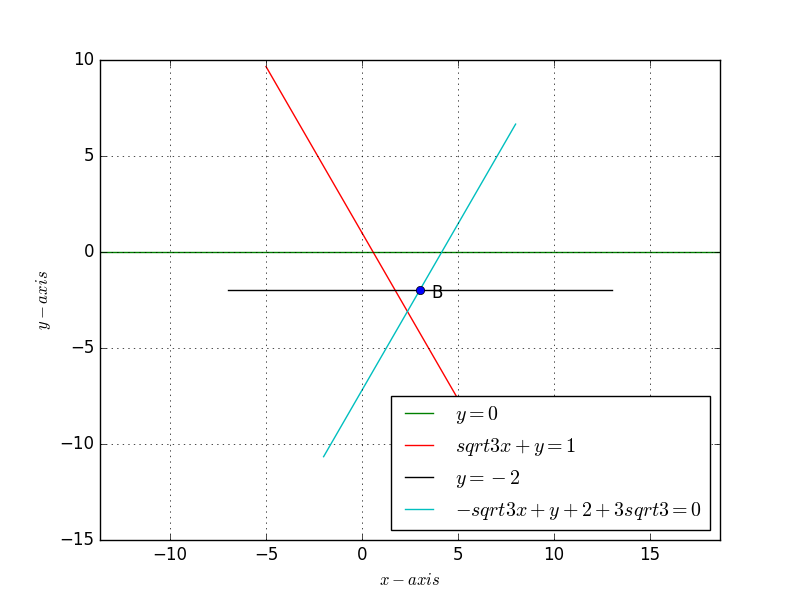
\includegraphics[scale=0.6]{FINAL.png}

\end{frame}
}

\end{document}
